\chapter{Welcome to the real world!}

\section{Signaux analogiques}
\subsection{Perturbations et imperfections}
Un signal analogique n'est pas si idéal que ça, plusieurs formes de perturbations peuvent se manifester comme le bruit, c'est à dire une variation aléatoire du signal autour de sa moyenne mais encore de l'offset, des pics, oscillation, ...\\
L'origine de ces perturbations vient de l'imperfection des composants. On en distingue trois types :
\begin{enumerate}
	\item Sources de bruit
	\item Dipôles parasites
	\item Couplages parasites
\end{enumerate}
Ainsi un bout de fil génèrera un bruit thermique, typique aux métaux.

\subsection{Rapport signal/bruit}
Afin de caractériser ce bruit, on a défini le \textit{signal-to-noise ration} :
\begin{equation}
	SNR = 20\log\left(\dfrac{V_{eff}(\text{signal utile + perturbation})}{V_{eff}(\text{perturbations})} \right)
\end{equation}
Celui-ci est exprimé en \textbf{dB} et doit être le plus élevé possible pour que les perturbations soient les plus négligeables possibles.

\subsection{Bruit}
Le bruit possède deux propriétés : la variation aléatoire du signal et l'origine interne du composant (processus physique fondamental). La conséquence du bruit est le \textit{"plancher" fondamental}. Celui-ci dénote le fait que le bruit ne peut être totalement éliminé et fixe une limite stricte à la précision de l'information.

\subsection{Dipôles parasites}
\textit{Des dipôles parasites sont des phénomènes physiques non désirés mais inévitables}, des effets secondaires qui sont modélisables sous la forme d'un dipôle électrique (comme une résistance accompagnant une self).\\
Les conséquences de ces dipôles parasites se font ressentir dans une limitation de vitesse de réponse (variation d'énergie dans les composants réactifs), des oscillations parasites (résonance du circuit LC ou encore des chutes de tension (résistives ou inductives)).


\subsection{Couplages}
Par définition "\textit{Coupage = parasites}". C'est la pollution d'un signal utile par un signal extérieur. A la différence du bruit, son caractère n'est pas forcément aléatoire et son origine est externe au composant.\\
Il existe plusieurs types de couplages :
\begin{description}
	\item[Galvanique]; par un conducteur commun
	\item[Inductif]; par un champ magnétique (f.e.m. induite (Lenz))
	\item[Capacitif]; par un champ électrique
	\item[Radiatif]; par une onde EM
\end{description}


\subsection{Conclusion}
Du à la complexité du monde réel, il faudra parfois approfondir le modèle pour tenir compte d'effets du deuxième ordre et faire de la \textit{compatibilité électromagnétique}\footnote{Problèmes de câblages, blindages, ...} (CEM).


\section{Résistances}
\subsection{Résistances ordinaires}
\subsubsection{Propriété d'une résistance réelle}
\begin{wrapfigure}[11]{l}{5.9cm}
	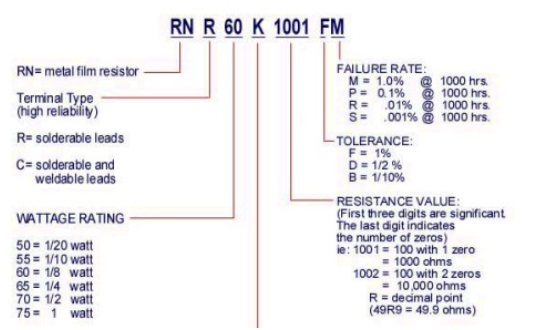
\includegraphics[scale=0.4]{img/image30.png}
	\captionof{figure}{Data-sheet d'une résistance}
\end{wrapfigure}
Il existe deux grands procédés de fabrication : les résistances à fil bobiné et les résistance au carbone.\\
Il est important de savoir que la résistance n'a pas pour seule propriété sa valeur ohmique, dictée par la loi d'Ohm $V = RI$. On retiendra ses limites d'utilisations :
\begin{itemize}
	\item Limite de puissance
	\item Limite de tension
	\item Limite de température
\end{itemize}
Au dela de ces limites, il faut également noter des écarts par rapport à la loi idéale, notamment la \textbf{tolérance} (précision sur $R$) et le coefficient de température ($R = f(T)$).

\subsubsection{Valeurs disponibles}
Afin de s'y retrouver, elles sont organisées en séries mais l'important est que l'on peut obtenir n'importe quelle valeur par mise en série et en parallèle. Le marquage de la résistance permet d'obtenir d'avantage d'informations sur celle-ci.

\subsubsection{Utilisation d'une résistance}
Avec une unique résistance, on retrouve les propriétés vue en électricité : conversion courant-tension, limitation du courant,  ... On peut également "découpler" des nœuds (permet que deux nœuds reliés soient à des potentiels différents) mais aussi de fixer le potentiel par défaut d'un nœud avec des résistance de pull-up et de pull-down.


\subsection{Résistances de puissance}
Le but d'une résistance de puissance est de dissiper une certaine puissance en pertes joules.

\subsection{Ajustables et potentiomètres}
\begin{wrapfigure}[9]{r}{3cm}
	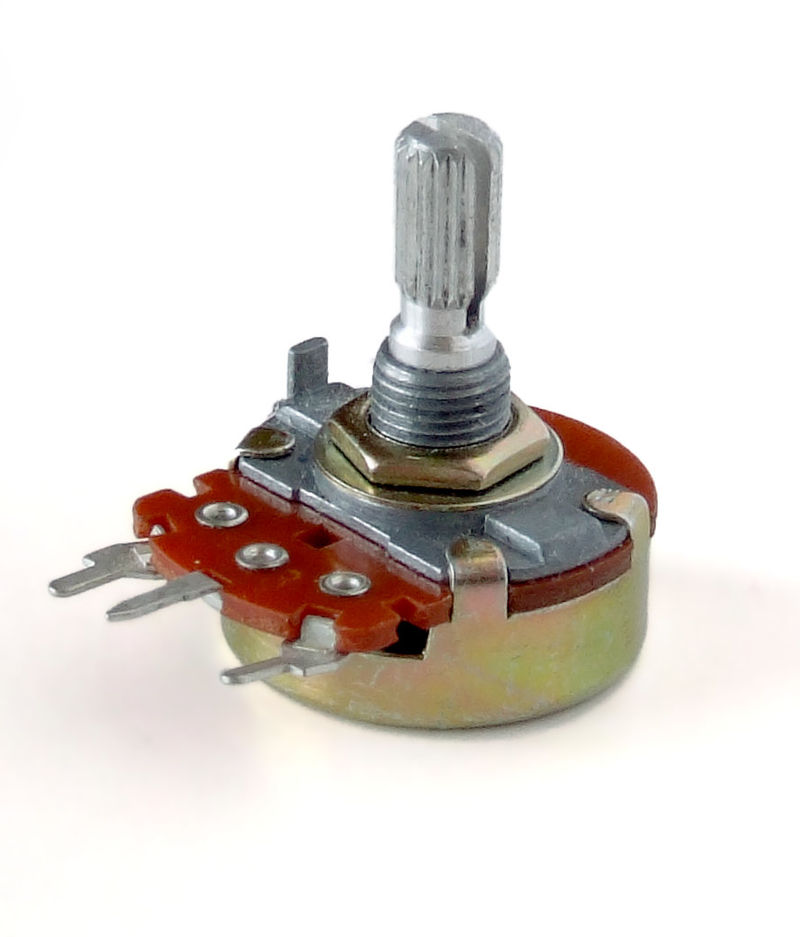
\includegraphics[scale=0.1]{img/image31}
	\captionof{figure}{Potentiomètre}
\end{wrapfigure}

Il s'agit de résistances variables, fonction de la position. Elles se composent de trois bornes et suivent une loi de variation. Leur ajustement peut par exemple se faire par tournevis.\\

Le \textit{potentiomètre} (ou \textit{potar}) est un type de résistance variable à trois bornes, dont une est reliée à un curseur se déplaçant sur une piste résistante terminée par les deux autres bornes. Ce système permet de recueillir, entre la borne reliée au curseur et une des deux autres bornes, une tension qui dépend de la position du curseur et de la tension à laquelle est soumise la résistance\footnote{Source : Wikipédia}.

\subsection{Autres types de résistance}
\subsubsection{Thermistance}
\begin{wrapfigure}[6]{l}{3cm}
	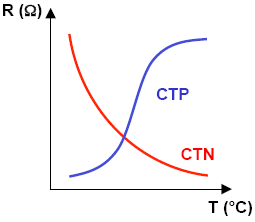
\includegraphics[scale=0.3]{img/image32}
	\captionof{figure}{Thermistance}
\end{wrapfigure}
La \textit{thermistance}, un résistance qui dépend de la température, faite en matériau semiconducteur. Son comportement est fortement non linéaire. Il en existe deux types :
\begin{enumerate}
	\item CTN - capteur de température de faible précision
	\item CTP - pour la protection
\end{enumerate}%\ \\

\subsubsection{Photorésistance}
Celle-ci se base sur le principe $LDR$ - \textit{light dependent resistor}. La résistance est fonction de l'éclairement ; elle est munie d'un capteur. 



\section{Condensateurs}
\subsection{Deux types de condensateurs}
La fonction $Q = CV$ définit la notion de \textit{capacité} qui n'est pas à confondre avec le composant réel : le \textit{condensateur}. Il en existe plus de vingt types différents, mais seulement deux familles : 
\begin{enumerate}
	\item Polarisés
	\item Non polarisés
\end{enumerate}

\subsection{Condensateurs non polarisés}
\begin{wrapfigure}[6]{r}{3cm}
	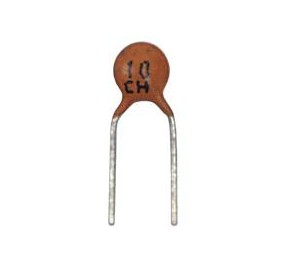
\includegraphics[scale=0.2]{img/image33}
	\captionof{figure}{Condensateur céramique}
\end{wrapfigure}
Ceux-ci n'ont pas de "sens" électrique préférable et sont généralement de "faible" valeur (du $pF$ au $\mu F$). Les "classiques" sont les condensateurs céramiques et ceux à films plastiques.\\

On les définit par leur capacité $C$, leur tension de service (50 à 400 $V$) et leur précision (maximum 10\%).

\newpage
\subsection{Condensateurs polarisés}
\begin{wrapfigure}[8]{l}{3cm}
	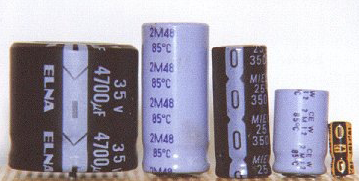
\includegraphics[scale=0.2]{img/image34}
	\captionof{figure}{Condensateurs polarisés}
\end{wrapfigure}
Ceux si possèdent un sens électrique (\textbf{risque d'explosion} si monté à l'envers !). Ils supportent une tension DC\footnote{Continue} ainsi qu'une faible composante AC\footnote{Alternative}. Son "sens" d'utilisation se discerne par une "bague".\\

Son principal avantage est de pouvoir stocker une énergie plus importante (coefficient de capacité de $1\mu F$ à quelques $mF$) mais au prix d'une précision médiocre (au mieux 20\%) et d'un encombrement non négligeable. Ceux-ci sont généralement de type électrochimique ($Al$) ou au tantale.


\subsection{Utilisations des condensateurs}
Rappelons que l'impédance d'un condensateur varie en fonction de la fréquence ("infinie" en continu et faible à HF). Il permet de "\textit{séparer}" le continu de l'alternatif. Plusieurs utilisations sont possible :
\begin{description}
	\item[Condensateur de liaison]; entre deux étages d'un montage, laisse passer l'alternatif (signal) mais bloque le continu( polarisation)
	\item[Condensateur de découplage ]; "court-circuite" un élément de polarisation en HF
	\item[Filtrage, réserve énergie, conversion charge-courant, ...]
\end{description}\ \\
Dans les circuits digitaux, on utilise des inductances pour de longues pistes en HF. Ces selfs causent des chutes de tension inductive (pics\footnote{A cause des commutations}) qui peuvent être absorbées par des condensateurs.\\
On utilisera les condensateurs non-polarisés comme "réserve locale" près des circuits (bon comportement en HF mais peu d'énergie) et préfèrera les polarisés (mauvais comportement HF mais beaucoup d'énergie) à l'entrée de montage pour compenser des variations lentes, mais importantes\footnote{A CLARIFIER}.

\subsection{Autres types de condensateurs}
Il existe également des condensateurs variables mais également des "supercapacités" de l'ordre du farad ! 


\section{Autres composants}
\subsection{Relais}

\textit{Un \textbf{relais} électromagnétique est un organe électrique permettant de dissocier la partie puissance de la partie commande  : Il permet l'ouverture/fermeture d'un circuit électrique par un second circuit complètement isolé (isolation galvanique) et pouvant avoir des propriétés différentes.}\footnote{Source : Wikipédia}\\

\begin{wrapfigure}[8]{r}{2cm}
	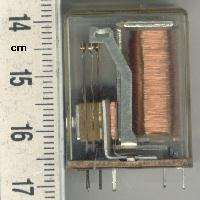
\includegraphics[scale=0.25]{img/image35}
	\captionof{figure}{Relais}
\end{wrapfigure}Le principe est donc celui d'un interrupteur commandable électroniquement, basé sur un électroaimant (l'interrupteur mécanique étant trop lent).\\
Son utilisation d'interface entre niveaux de puissances différents permet de commander une grosse puissance au moyen d'une petite (TWSS).


\section{Circuits imprimés}
Un circuit imprimé (PCB - \textit{Printed circuit board}) est un support permettant de relier électriquement un ensemble de composants électroniques. Il ne faut \textbf{pas} le confondre avec un circuit intégré.\\
Ces plaques, recouvertes de substrats isolants sont munies de couches conductrices par gravure chimiques. 


\section{Types de composants}
\subsubsection{Composants classiques >< SMD}
Les composants \textbf{classiques} traversent le substrat et la soudure se fait du côté opposé au composant. Les composants à \textbf{montage de surface} utilisent le SMD (\textit{Surface mount device}), un collage et soudure du même coté du PCB. Cela permet des composants très miniaturisés mais bonne chance pour les réparations.


\subsubsection{Composants discrets >< intégrés}
Les composants \textbf{discrets} ne réalisent qu'une fonction élémentaire unique (R, L, C, diode, transistor, ...) alors que les composants \textbf{intégrés} comportent généralement une "puce" composée de beaucoup de transistors et ayant des fonctions plus ou moins complexes (AOP, microprocesseur, ...).
